\documentclass{report}

\title{\Large{\textbf{TMA template file}}}
\author{First-name Surname {\textbf{OU ID \#}}}
\date{\today}

%\usepackage[margin=0.5in]{geometry}
\usepackage{pgfplots}
\usepackage{mathtools}
\usepackage{cancel}
\usepackage{pgfplots}
\usepackage{amsmath}
\newtheorem{theorem}{THEOREM}
\newtheorem{proof}{PROOF}
\usepackage{tikz}
\usetikzlibrary{arrows}
\usepackage{amssymb}
\usetikzlibrary{patterns}
\usepackage{bigints}
\usepackage{color}
\usepackage{tcolorbox}
\usepackage{booktabs,array}
\usepgfplotslibrary{fillbetween}

\usepackage{amsmath}
\usepackage{index}
\usepackage{fancyhdr}
%\usepackage{tikzpicture}
\usepackage{pgfplots}
%\usepackage{pifont}
%usepackage{xltxtra,xunicode}
\usepackage{soul,xcolor}
\makeindex
\usepackage{enumerate}

\pgfplotsset{compat=1.16}

\begin{document}

\begin{titlepage}
\maketitle
\end{titlepage}

\tableofcontents
\pagebreak

\pagenumbering{arabic}

\pagestyle{fancy}
\fancyhf{}
\rhead{Overleaf}
\lhead{MU123 19B}
\rhead{forename surname OU ID}
\rfoot{Page \thepage}
\lfoot{TMA \#}

%start working after this
\chapter{Chapter 1 Drawing Examples}

\subsection*{Source code here}

\subsection*{Strikethrough text}
\setstcolor{red}

\st{Some overstruck text}

\[ \frac{\cancel{3}.4^{n+1}}{\cancel{3}}\\ \]

\section{Drawing things}

\subsubsection{Draw a plain line}
 See fig:\ref{Example line drawing}
\begin{figure}[ht]
\begin{tikzpicture}
% Draw a line
\draw (0,0) -- (4,0);
\end{tikzpicture}
\caption{Example line drawing}
\label{Example line drawing}
\end{figure}



To draw a rectangle state the size x,y as shown in fig:\ref{Example rectangle drawing}

\begin{figure}[ht]
\begin{tikzpicture}
%\subsubsection{Draw a rectangle}
\draw (0,0) -- (6,0) -- (6,4) -- (0,4) -- cycle;
\end{tikzpicture}
\caption{Example rectangle drawing}
\label{Example rectangle drawing}
\end{figure}

To draw a parabola, state the co-ordinates as found in fig:\ref{Example parabola drawing}

\begin{figure}[ht]
\begin{tikzpicture}
% \draw (0,0) rectangle (6,4);
\draw (0,0) parabola (6,4);
\end{tikzpicture}
\caption{Example parabola drawing}
\label{Example parabola drawing}
\end{figure}

\subsection{inequalities}
An example of an inequality may be found in fig:\ref{example inequality}

\begin{figure}[ht]
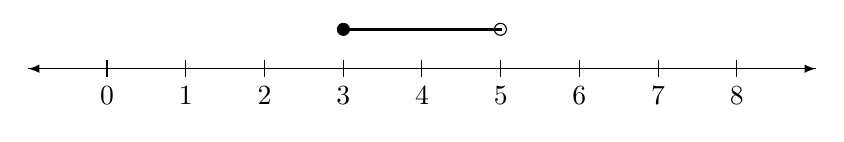
\begin{tikzpicture}
\draw[latex-] (-1,0) -- (9,0) ;
\draw[-latex] (-1,0) -- (9,0) ;
\foreach \x in  {0,1,2,3,4,5,6,7,8} \draw[shift={(\x,0)},color=black] (0pt,3pt) -- (0pt,-3pt);
\foreach \x in {0,1,2,3,4,5,6,7,8} \draw[shift={(\x,0)},color=black] (0pt,0pt) -- (0pt,-3pt) node[below] {$\x$};
\draw[*-o] (2.92,0.5) -- (5.08,0.5);
% * means includes (full circle), and o means excludes (empty circle)
\draw[very thick    ] (2.98,0.5) -- (5.02,0.5);
\end{tikzpicture}	
\caption{example inequality}
\label{example inequality}
\end{figure}


\begin{comment}
\subsubsection*{Source code here}
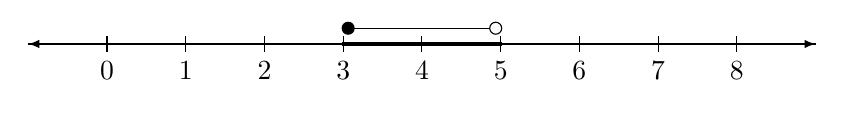
\begin{tikzpicture}
\draw[latex-] (-1,0) -- (9,0) ;
\draw[-latex] (-1,0) -- (9,0) ;
\foreach \x in  {0,1,2,3,4,5,6,7,8} \draw[shift={(\x,0)},color=black] (0pt,3pt) -- (0pt,-3pt);
\foreach \x in {0,1,2,3,4,5,6,7,8} \draw[shift={(\x,0)},color=black] (0pt,0pt) -- (0pt,-3pt) node[below] {$\x$};
\draw[*-o] (2.98,0.2) -- (5.02,0.2);
% * means includes (full circle), and o means excludes (empty circle)
\draw[very thick    ] (2.98,0) -- (5.02,0);
\end{tikzpicture}	
	
\end{comment}

\subsection{factor trees}

An example of simple factor tree can be seen on the pages below in fig:\ref{Factor tree simple}
\begin{figure}[!hb]
    \centering
    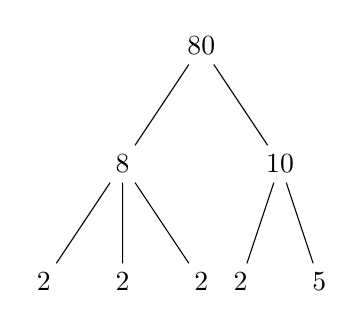
\begin{tikzpicture}[
        level 1/.style={sibling distance=20mm},
        level 2/.style={sibling distance=10mm},
    ]
    \node{80}
        child{node {8}
            child{node {2}}
            child{node {2}}
            child{node {2}}
        }
        child{node {10}
            child{node {2}}
            child{node {5}}
        };
    \end{tikzpicture}
    \caption{Simple tree}
    \label{Factor tree simple}
\end{figure}

An example of an elaborated factor tree can be seen below in fig:\ref{Factor tree elaborate} 

\begin{figure}[!ht]
    \centering
    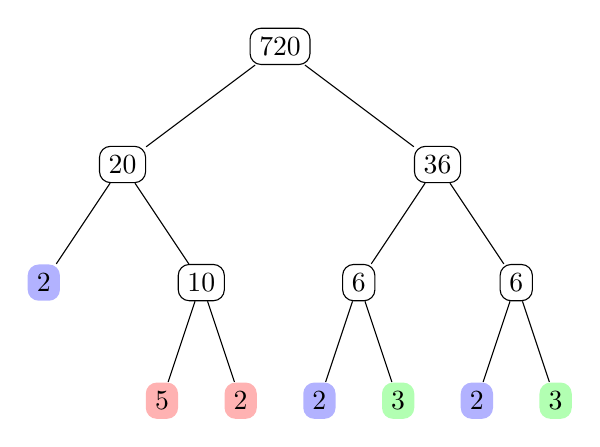
\begin{tikzpicture}[
        level 1/.style={sibling distance=40mm},
        level 2/.style={sibling distance=20mm},
        level 3/.style={sibling distance=10mm}
        ]
    \node[rounded corners, draw]{720}
        child{node [rounded corners, draw] {20}
            child{node [fill=blue!30,rounded corners] {2}}
            child{node [rounded corners, draw] {10}
                child{node [fill=red!30,rounded corners] {5}}
                child{node [fill=red!30,rounded corners] {2}}
            }
        }
        child{node [rounded corners, draw] {36}
            child{node [rounded corners, draw] {6}
                child{node [fill=blue!30,rounded corners] {2}}
                child{node [fill=green!30,rounded corners] {3}}
            }
            child{node [rounded corners, draw] {6}
                child{node [fill=blue!30,rounded corners] {2}}
                child{node [fill=green!30,rounded corners] {3}}
            }
        };
    \end{tikzpicture}
    \caption{Elaborated tree}
\label{Factor tree elaborate}
\end{figure}

\clearpage

\subsection{Graphs}
an example of a graph may be seen in \ref{A Graph}

\begin{figure}[!h]
	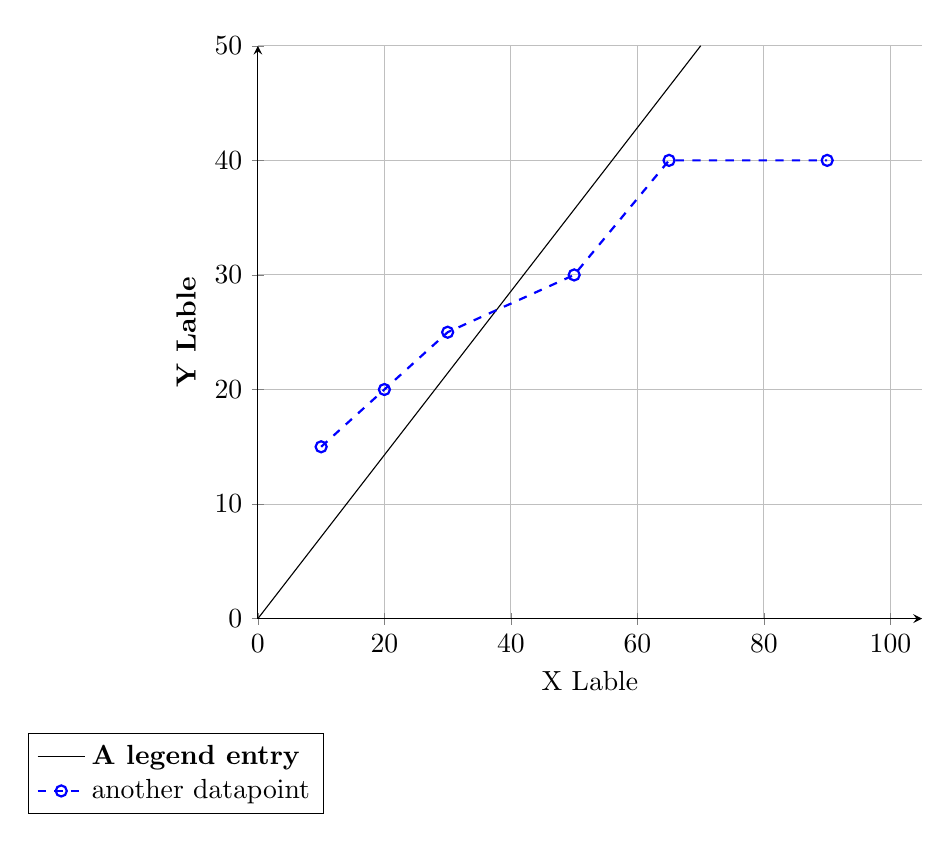
\begin{tikzpicture}

	\begin{axis}[%
	%state where you want your legend to go setting below result in bottom center
	legend style={
            at={(0.1,-0.2),anchor=north}
        },
	% State the axis scale        
	compat=newest,
	scale only axis,
	xmin=0, xmax=105,
	xlabel={\text{X Lable}},
	xmajorgrids,
	ymin=0, ymax=50,
	ylabel={\textbf{Y Lable}},
	ymajorgrids,
	axis lines=left,
	title={ },
	legend style={nodes=right}]
	% Set up your data set
	\addplot [
		color=black,
		solid
	] coordinates {(0,0) (70,50)};
	\addlegendentry{\textbf{A legend entry}};
	% Set up your data set
	\addplot[mark=o,mark options={solid},blue,thick,dashed] coordinates {
        (10,15)	(20,20) (30,25) (50,30) (65, 40) (90,40)};
    \addlegendentry{another datapoint}
	\end{axis}
	\end{tikzpicture}
	%What I tell you right now may save you hours of extensive debugging, cursing under your breath, commenting out custom code dealing with figure layout and much frustration. Whenever you use figures, always (and I mean ALWAYS EVER FOREVER ALWAYS) put \caption first, and \label second like this:
	\caption{example graph}
	\label{A Graph} 
\end{figure}

\clearpage

\subsection{Tables}

\begin{center}
\begin{tabular}{c c}
Col 1a & Col 2a \\
Col 2b & Col 2b \\
Col 3c & Col 3c \\
Col 4d & Col 4d \\
\end{tabular}
\end{center}

\begin{table}

\begin{center}
\begin{tabular}{|c|c|c|}
\hline
\multicolumn{1}{|c|}{} & \multicolumn{2}{c|}{dataset} \\
					\cline{2-3}
Col 1a & Col 2a & Col 3a \\
\hline
Col 2b & Col 2b & Col 3b \\
\hline
Col 3c & Col 3c & Col 3c \\
\hline
Col 4d & Col 4d & Col 3d \\
\hline
\end{tabular}
\end{center}
\label{table2}
\caption{This is a more detailed column}
\end{table}

\chapter{Chapter 2 formating}
\section{Unit x}

\subsection{Strategy - details}

\subsection{Activity - details}

\subsubsection{(a) - question details}

\begin{itemize}
\item[i] specifics about the question
\item[ii] specifics about the question
\item[iii] specifics about the question
\end{itemize}
\clearpage

\section{Alternative markup} %useful if writing up subchapters or questions, will not update the TOC, alghou this can be done manually. I am not going into is as I have no intention on doing so in this iteration.

\begin{enumerate}
	\item Arabic
	\item Arabic
	\begin{enumerate}[(a)]% square brackets define the itemlist type and format this example includes brackets
		\item Alpha
			\begin{enumerate}[(i)]
				\item Roman
			\end{enumerate}
		\item next sub section
			\begin{enumerate}[(i)]
				\item example 1
				\item anonther part question answer or referance
			\end{enumerate}	
	\end{enumerate}
	\item referancing another subsection Figure:\ref{A Graph}
\end{enumerate}

\section{set enumerate count}
\begin{enumerate}[4] % this overrides the enumerate count, this will cause an error "The counter will not be printed. try format documents to autocount as this makes indexing and referancing easier see "https://tex.stackexchange.com/questions/119719/add-an-item-in-the-table-of-contents" for more info
	\item arabic
	\begin{enumerate}
		\item alpha
			\begin{enumerate}
				\item roman
				\item next item
			\end{enumerate}
		\item next alpha			
	\end{enumerate}
	\item next arabic
\end{enumerate}

N.B. this does not create a Table Of Contents, you would need to use "section" to build this out, additionally the enumerate value will overide the count see difference between the first and second example.

The counter will not be printed warnings refer to the enumerate value being specified.
\clearpage


\end{document}